\documentclass[10pt]{article}
\usepackage[letterpaper, margin=1in]{geometry}
\usepackage[pdftex]{graphicx}
\usepackage[utf8]{inputenc}
\usepackage{tikz, wrapfig, amssymb, array, mathtools, circuitikz, physics, parskip, hyperref}
\usepackage{enumerate}
\usepackage{tkz-euclide}
\usepackage{titlesec}
\usepackage{lipsum}
\usepackage[english]{babel}
\usepackage{amsmath, amsthm}
\usepackage{fancyhdr}
\usepackage{xcoffins}
\usepackage{tcolorbox}
\usepackage{../local}


\newcommand{\classcode}{Physics 5C}
\newcommand{\classname}{Introductory Thermodynamics and Quantum Mechanics}
\renewcommand{\maketitle}{%
\hrule height4pt
\large{Eric Du \hfill \classcode}
\newline
\large{HW 06} \large{\hfill \classname \hfill} \large{\today}
\hrule height4pt \vskip .7em
\normalsize
}
\linespread{1.1}
\begin{document}
    \maketitle

    \section*{Collaborators}

    I worked with (in no particular order) \textbf{Andrew Binder, Aren Martinian, Nathan Song, Christine Zhang, Nikhil Maserang} and \textbf{Teja Nivarthi} to complete this homework assignment.
    \section*{Problem 1}

    A neutral uranium atom has 92 electrons surrounding a nucleus containing 92 protons. 


    \begin{enumerate}[(a)]
        \item Given that the Bohr radius for the lowest energy in hydrogen is $a_0 = 0.5$ \AA, derive an approximate numerical value on the basis of mechanics for the radius of the smallest Bohr orbit about the uranium nucleus.
        
        \begin{solution}
            By Coulomb's Law and centripetal force, we have that 

            \[ \frac{kq_1q_2}{r^2} = \frac{mv^2}{r} \implies r = \frac{kq_1q_2}{mv^2}\]

            From Bohr's hypothesis we know that angular momentum is quantized, so $L = mvr = \hbar n$. We claim that the expression of the angular momentum for the uranium atom is the same as that for the hydrogen atom. Using angular momentum, we can derive the equation: 

            \[ L^2 = (mvr)^2 = \frac{kq_1q_2mr^2}{n^2\hbar^2} \implies r = \frac{n^2 \hbar^2}{m kq_1q_2}\]

            For hydrogen, we know that we have one electron and one proton of the same charge, so $qQ = e^2$. Therefore, this gives us $r_H = \frac{n^2\hbar^2}{ke^2m} = 0.5$\AA  given from the problem. We then know that for uranium, there are 92 protons, so therefore $q_1q_2 = 92e^2$ so therefore 

            \[ r_U = \frac{n^2\hbar^2}{92ke^2m} = \frac{1}{92}r_H\]

            And so we derive the fact that the uranium atom is about 1/92 the size of that of a hydrogen atom. 
        \end{solution}
        \item In a violent nuclear event a uranium nucleus is stripped of all 92 electrons. The resulting bare nucleus captures a single free electron fron the surroundigns. Given that the ionization energy for hydrogen is 13.6 eV, derive an approximate numerical value for the maximum energy of the photon that can be given off as the uranium nucleus captures this first electron.
        
        \begin{solution}
            We know the initial energy $E_i = 13.6$ eV for Hydrogen, given by the problem statement. Since the total energy of a hydrogen atom is just the sum of its potential and kinetic energy: 

            \[ E_i = \frac{1}{2}mv^2 + \frac{kq_1q_2}{r_H}\] 

            and we have $\frac{mv^2}{r} = \frac{kq_1q_2}{r^2}$ then combining these two equations we get: 

            \[ E = \frac{3}{2} \frac{kq_1q_2}{r_H}\]

            Again, from the last part we know that $q_1q_2 = 92e^2$ so therefore, 

            \[ E_U = \frac 32 \frac{92 ke^2}{\frac{1}{92}r_H} = 92^2 E_H = 1.15 \times 10^5 \text{ eV}\]


        \end{solution}
        \item Calculate the value of $v/c$ for the frist Bohr orbit in $\text{U}^{92}$ according to Newtonian mechanics. This will show you that relativistic dynamics should really be used in this problem.
        
        \begin{solution}
            We know from angular momentum:

            \[ L = mvr = n\hbar \implies v = \frac{n\hbar}{mr} = 2.12 \times 10^8\] 

            Therfore, $v/c \approx 0.71$, so relativistic dynamics should be used in this problem.
        \end{solution}
    \end{enumerate}


    \pagebreak
    \section*{Problem 2}

    A rough criterion for the applicability of ordinary particle mehcanics (either Newtonian or relativistic) is that the de Broglie wavelength be much less than some characteristic linear dimension $l$ of the system. For $l \lesssim \lambda$, wave mechanics is needed. Apply these criteria to the following systems


    \begin{enumerate}[(a)]
        \item \textit{Electtron in the atom.} Use the de Broglie relation to calculate $\lambda/r$ for the electron in the first Bohr orbit of hydrogen. Does your result veirfy that we need to use quantum physics to describe the behavior of electrons in atoms?
        
        \begin{solution}
            We know that $E = \frac{hc}{\lambda}$, then we also get $\lambda = \frac{hc}{E} = 9.14 \times 10^{-8}$ m. Calculating the ratio of $\lambda/r$:

            \[ \frac{\lambda}{r} = \frac{9.19 \times 10^{-8}}{0.5 \times 10^{-10}} = 1830\] 

            Since $r < \lambda$, then quantum mechanics is needed. 
        \end{solution}
        \item \textit{Proton in the nucleus.} Assume that one of the protons in a large nucleus (nuclear radius $\approx 10^{-12}$ cm) is in a circular orbit inside the nucleus with kinetic energy 10 MeV. Calculate $\lambda/r$ for the orbiting proton. Do we need quantum phsycis to descrbe this nuclear system?
        
        \begin{solution}
            Again we use the same equation: $\lambda = \frac{hc}{E}$. Writing out the energy:

            \[ E = \frac{kq_1q_2}{r} + \frac 12 mv^2 \]

            so using the relation that $\frac{mv^2}{r} = \frac{kq_1q_2}{r^2}$ we then get:

            \[E = mv^2 + \frac{1}{2} mv^2 = 3 \cdot \text{KE}\]

            And so therefore 

            \[ \lambda = \frac{hc}{3 \text{KE}} \approx 4.14 \times 10^{-14} \text{ m}\]

            Calculating $\lambda/r$: 

            \[ \frac \lambda r = \frac{4.14 \times 10^{-14}}{10^{-14}} = 4.14\] 

            So since $r \lesssim \lambda$, quantum mechanics is needed here as well.

        \end{solution}
        \item \textit{Electrons in a TV set.} The electrons in a typical television receiver have kinetttic energies of the ordder of 10 keV. Do the designers of the image-forming systetms in television sets have to use quantum physics in their calculations? 

        \begin{solution}
            Same equation: 

            \[ \lambda = \frac{hc}{E} \approx 1.24 \times 10^{-10} \text{ m}\]

            Here, however, the characteristic length for a TV receiver is likely on the order of 1m, so therefore $l \ll \lambda$, and so therefore quantum mechanics is not needed here.
        \end{solution}
    \end{enumerate}


    \pagebreak
    \section*{Problem 3}

    The Lyman alpha radiation for hydrogen (resulting from the transition $n = 2$ to $n = 1$) has a wavelength in the ultraviolet, $1216.0$ \AA. Using the crude model of the one-dimensional infinite square well, derive an estimate of the diameter of a hydrogen atom. How does this value compare with twice the Bohr radius, $2a_0 = 1.06$ \AA?

    \begin{solution}
        The energy levels for the infinite square well are given by: 

        \[ E_n = \frac{(\hbar n \pi)^2}{2mL^2}\] 

        We know that the electron goes from $n = 2$ to $n = 1$, so therefore we have 

        \[ E_2 - E_1 = E_{light} = \frac{hc}{\lambda}\]

        Therefore 

        \begin{align*}
            E_2 - E_1 &= 3\left(\frac{\pi^2 \hbar^2\pi^2}{2 mL^2}\right) = \frac{hc}{\lambda}\\
            \therefore L &= \left(\frac{3 \pi \hbar \lambda}{4 mc}\right)^{1/2} \approx 3.32 \times 10^{-10} \sim 3 \text{\AA}
        \end{align*}

        This is approximately 3 times larger than the Bohr radius, which is not a terrible approximation, but also not great either.
    \end{solution}
    \pagebreak
    \section*{Problem 4}

    The boundary between the interior of a metal and the air or vaccuum may be modeled by a rectangular potential step, as shown in the figure. The height of the potential step ($V_n$) exteeds the energy of the most energetic conduction electrons ($E$). The difference $V_0 - E$ is called the work function, $W$.

    \begin{center}
        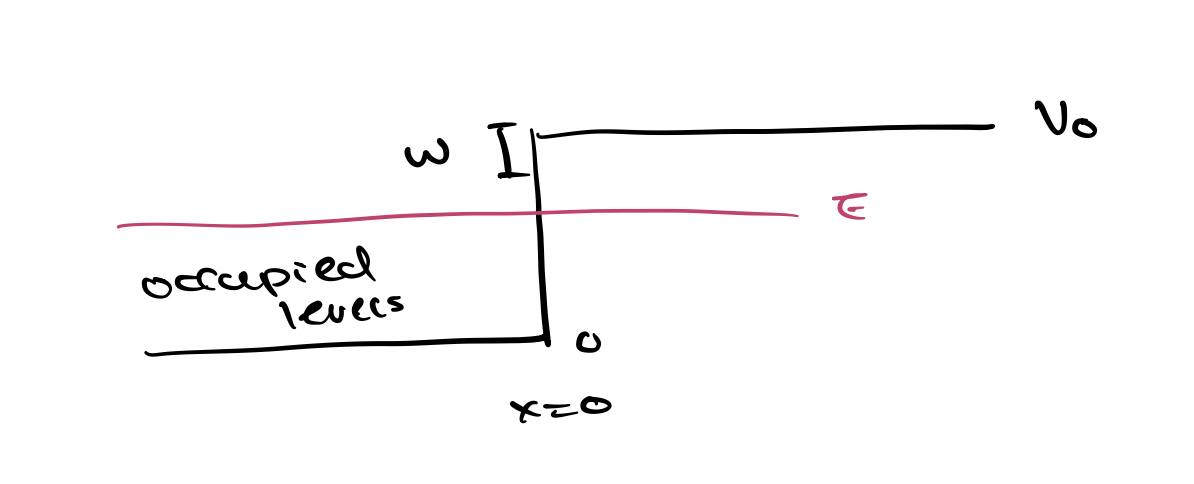
\includegraphics[scale=0.5]{potential.png}
    \end{center}

    \begin{enumerate}[(a)]
        \item What is the form of the wave function outside the metal for the electrons that are most energetic? What is the form of the function that describes the probability density of finding these electrons ta a given distance outside the surface?

        \begin{solution}
            For locations at $x > 0$, we know we need an evanescent wave, so therefore 

            \[ \psi(x) = Ae^{-\alpha x}\]

            Therefore, the probability density is given by 

            \[ P(x) = |\Psi(x)|^2 = A^2e^{-2\alpha x}\]
        \end{solution}
        \item Assume that the work function is 5 eV. Estimate the distance outsdie the metal at which the probability density function drops to a fraction $(1/e)^7 \approx 1/1000$ of that just inside the metal.
        
        \begin{solution}
            The probability density is given by $P(x) = |\psi(x)|^2$ so therefore 

            \[ |\psi(x)|^2 = A^2e^{-2\alpha x}\]

            The probability density just inside the metal can be thought of as $P(0) = A^2e^{-2\alpha(0)} = A^2$ so therefore we have :

            \begin{align*}
                A^2e^{-2\alpha x} &= \frac{1}{e^7} A^2\\
                2\alpha x &= -7 \\
                x \approx 3.05 \times 10^{-10} \text{ m}
            \end{align*}
        \end{solution}
        \item Compare the distance estimated in part (b) with an estimate of the minimum roughness of a polished metal surface over comparable distances. How useful do you expect the "step-potential" model of a surface of a metal to be?
        
        \begin{solution}
            The estimated distance of the minimal roughnes of a polished metal is about 1nm, so therefore the step potential being smaller (1/10th of the size) on these scales would make sense. It is also a useful approximation in this case because not only does it make physical sense but the energy eigenfunctions are also easy to find.       
        \end{solution} 
    \end{enumerate}


    \pagebreak

    \section*{Problem 5}

    The text states that, in one-dimensional problems, the spatial wave function for any allowed state can be chosen to be real-valued. Verify this using the following outline or some other method. 

    \begin{enumerate}[(a)]
        \item Write the wave function $\psi_n(x)$ in terms of its real and imaginary parts: $\psi_n = \Re(\psi_n) + i \Im(\psi_n)$, and substitute this into the \schrodinger equation.
        \item Show that $\Re \psi_n$ and $\Im \psi_n$ separately satisfy the \schrodinger equation.
        \item In one dimension there is only one (linearly independent) wave function for each energy eivenvalue $E_n$. What does this imply about $\Re \psi_n$ and $\Im \psi_n$? Describe how you can construct a real, normalized wave function from $\psi_n$.
    \end{enumerate}

    \begin{solution}
        We will use an alternate solution. Suppose that $\psi(x)$ satisfies the \schrodinger equation:
        \[ -\frac{\hbar^2}{2m}\frac{d^2\psi}{dx^2} + V\psi = E\psi\]

        If this is true, then the conjugate $\psi^\star$ also satisfies the \schrodinger equation:

        \[-\frac{\hbar^2}{2m}\frac{\partial^2\psi^{\star}}{dx^2} + V\psi^\star = E\psi^{\star}\]

        Now since $\psi$ and $\psi^\star$ satisfy the \schrodinger equation, then any linear combination of these two will also be solutions to the \schrodinger equation, since it is a linear equation. Thus, $(\psi + \psi^{\star})$ and $i(\psi - \psi^{\star})$ will also be solutions to the \schrodinger equation. Since these solutions will be real, then we can always write it as a linear combination of real solutions, and hence $\psi(x)$ can always be taken to be real.
    \end{solution}
    \pagebreak
    
    \section*{Problems 6 and 7}

    These problems are attached below: 
\end{document}